% !TeX spellcheck = en_GB
% !TeX program = pdflatex
%
% LuxSleek-CV 1.1 LaTeX template
% Author: Andreï V. Kostyrka, University of Luxembourg
%
% 1.1: added tracking and letter-spacing for prettier lower caps, added `~` for language levels
% 1.0: initial release
%
% This template fills the gap in the available variety of templates
% by proposing something that is not a custom class, not using any
% hard-coded settings deeply hidden in style files, and provides
% a handful of custom command definitions that are as transparent as it gets.
% Developed at the University of Luxembourg.
%
% *NOTHING IS HARCODED, and never should be.*
%
% Target audience: applicants in the IT industry, or business in general
%
% The main strength of this template is, it explicitly showcases how
% to break the flow of text to achieve the most flexible right alignment
% of dates for multiple configurations.

\documentclass[11pt, a4paper]{article} 

\usepackage[T1]{fontenc}     % We are using pdfLaTeX,
\usepackage[utf8]{inputenc}  % hence this preparation
\usepackage[british]{babel}  
\usepackage[left = 0mm, right = 0mm, top = 0mm, bottom = 0mm]{geometry}
\usepackage[stretch = 25, shrink = 25, tracking=true, letterspace=30]{microtype}  
\usepackage{graphicx}        % To insert pictures
\usepackage{xcolor}          % To add colour to the document
\usepackage{marvosym}        % Provides icons for the contact details

\usepackage{enumitem}        % To redefine spacing in lists
\setlist{parsep = 0pt, topsep = 0pt, partopsep = 1pt, itemsep = 1pt, leftmargin = 6mm}

\usepackage{FiraSans}        % Change this to use any font, but keep it simple
\renewcommand{\familydefault}{\sfdefault}

\definecolor{cvblue}{HTML}{304263}

%%%%%%% USER COMMAND DEFINITIONS %%%%%%%%%%%%%%%%%%%%%%%%%%%
% These are the real workhorses of this template
\newcommand{\dates}[1]{\hfill\mbox{\textbf{#1}}} % Bold stuff that doesn’t got broken into lines
\newcommand{\is}{\par\vskip.5ex plus .4ex} % Item spacing
\newcommand{\smaller}[1]{{\small$\diamond$\ #1}}
\newcommand{\headleft}[1]{\vspace*{3ex}\textsc{\textbf{#1}}\par%
    \vspace*{-1.5ex}\hrulefill\par\vspace*{0.7ex}}
\newcommand{\headright}[1]{\vspace*{2.5ex}\textsc{\Large\color{cvblue}#1}\par%
     \vspace*{-2ex}{\color{cvblue}\hrulefill}\par}
%%%%%%%%%%%%%%%%%%%%%%%%%%%%%%%%%%%%%%%%%%%%%%%%%%%%%%%%%%%%

\usepackage[colorlinks = true, urlcolor = white, linkcolor = white]{hyperref}

\begin{document}

% Style definitions -- killing the unnecessary space and adding the skips explicitly
\setlength{\topskip}{0pt}
\setlength{\parindent}{0pt}
\setlength{\parskip}{0pt}
\setlength{\fboxsep}{0pt}
\pagestyle{empty}
\raggedbottom

\begin{minipage}[t]{0.33\textwidth} %% Left column -- outer definition
%  Left column -- top dark rectangle
\colorbox{cvblue}{\begin{minipage}[t][5mm][t]{\textwidth}\null\hfill\null\end{minipage}}

\vspace{-.2ex} % Eliminates the small gap
\colorbox{cvblue!90}{\color{white}  %% LEFT BOX
\kern0.09\textwidth\relax% Left margin provided explicitly
\begin{minipage}[t][293mm][t]{0.82\textwidth}
\raggedright
\vspace*{2.5ex}

\Large Senior Software Engineer \textbf{\textsc{Ludovic Aubert}} \normalsize 

% Centering without extra vertical spacing
\null\hfill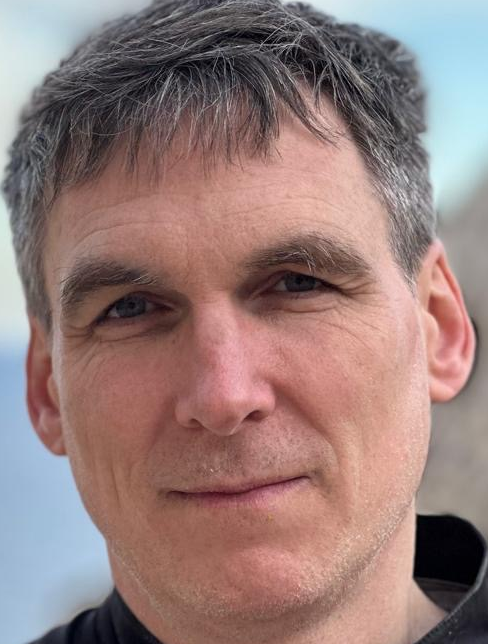
\includegraphics[width=0.65\textwidth]{lax.png}\hfill\null

\vspace*{0.5ex} % Extra space after the picture

\headleft{Project}
I hold an Engineering degree from the Ecole Centrale in Paris and combine a strong background in Mathematics with 25 years of experience working on diversified software and data projects. In the first period of my career, I mostly worked on C++ projects, some of which required algorithmic design. In the second period, I mostly worked on Data projects. I am looking for complex and critical projects using a mix of data, software and web technologies.

\headleft{Contact}
\small % To fit more content
\MVAt\ {\small ludo.aubert@gmail.com} \\[0.4ex]
\Mobilefone\ 06\,68\,40\,98\,26\ \\[0.5ex]
\Mundus\ \href{https://github.com/ludoaubert}{github.com/ludoaubert} \\[0.1ex]

\headleft{Languages}
\textbf{Francais}~(native), \textbf{Espagnol}~(B1), \textbf{Allemand}~(C2), \textbf{Anglais}~(C2)

\headleft{Skills}
\begin{itemize}
\item C++, SQL, CSS
\item Javascript, JSON, HTML
\item SQL Server, PostgreSQL, Oracle
\item NodeJS
\item Communication and team collaboration
\end{itemize} 

\end{minipage}%
\kern0.09\textwidth\relax%%Right margin provided explicitly to stretch the colourbox
}
\end{minipage}% Right column
\hskip2.5em% Left margin for the white area
\begin{minipage}[t]{0.56\textwidth}
\setlength{\parskip}{0.8ex}% Adds spaces between paragraphs; use \\ to add new lines without this space. Shrink this amount to fit more data vertically

\vspace{2ex}

\headright{Réalisations}

\textsc{Senior software engineer} at \textit{Ipside (La Defense).}  \dates{2021--2025} \\

\textsc{Patent database schema migration and merge} \\
\smaller{. I performed the migration into a new schema and merger of patent databases during a company acquisition. This initiative saved hundreds of thousands in cloud costs, streamlined data management, and supported the integration of three companies, valued in millions.}

\textsc{Patent inventor deduplication process} \\
\smaller{Developed a graph algorithm to deduplicate inventor data, consolidating multiple records into a single inventor table. Successfully created a table with 16,000 unique inventors,improving data reliability.}

\textsc{Extraction of 4 million documents} \\
\smaller{Wrote scripts and ran the extraction of 4TB of archived corporate documents from Oracle (files stored in DB) into the filesystem.}

\textsc{developed a module using C++} \\
\smaller{development functionality to create a directory structure to store legal documents on the migration target system. The structure depends on a set of parameters specific to a patent.}

\textsc{Prototype development of a patent web interface} \\
\smaller{Created a Proof of concept using NodeJS and new SQL JSON capabilities to navigate the patent database in a web browser. Developed a quick prototype of web interface to navigate patent information.}

\is
\textsc{Senior Software Engineer} at \textit{Paprec} \dates{2019--2020} \\

\textsc{Plastic recycling plants traceability graph} \\
\smaller{I fixed a script to generate traceability graphs for six plastic recycling plants. I suggested rewriting the script, which was accepted, and I developed a more efficient and reliable version using advanced SQL features, resulting in scalable solution that produced up to 6 million rows.}

\textsc{Flexible HR database with tracking} \\
\smaller{Design from scratch of a motivation and tracking database for HR. Due to integration of COVED, PAPREC needs a more flexible database design. Design of a test prototype to validate the structure. Integration of paid vacation trackers with a 3 year record.}

\textsc{ELT for Massive geographic data} \\
\smaller{Paprec ESRI Geographic Data Hub. Development of a SQL+python ELT to transfer GBytes of data hosted by various providers such as Kizeo, Novacom, Simpliciti, Sigrenea for Paprec into a geographic database hosted on the corporate infrastructure.}

\headright{Education}

\textsc{Engineering Degree with Major in Software and Electronics} \\\textit{Ecole Centrale de Paris}. \dates{1992--1996}

\textsc{Preparatory School with focus on Maths} \\
\textit{Lycee Sainte Genevieve}.  \dates{1990--1992}

\headright{Hobby}

\textsc{Bike trip and camping: Paris to Barcelona, 8 days}
\smaller{I accompanied my son, riding 120 km dayly, ensuring the trip ran smoothly within a budget of 10 euros per day.}

\end{minipage}

\end{document}
